\section{Chandra Kirana Poetra (1174079)}
\subsection{Membaca Shapefile dengan PySHP}
\begin{enumerate}
	\item Nomor 1
	\lstinputlisting{src/tugas3/1174079/soalno1.py}
	\begin{figure}[H]
		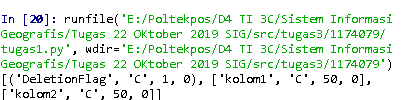
\includegraphics[width=6cm]{figures/Tugas3/1174079/soal1.png}
		\centering
		\caption{Gambar Soal 1}
	\end{figure}
	\item Nomor 2
	\lstinputlisting{src/tugas3/1174079/soalno2.py}
	\begin{figure}[H]
		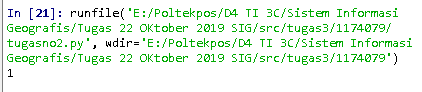
\includegraphics[width=6cm]{figures/Tugas3/1174079/soal2.png}
		\centering
		\caption{Gambar Soal 2)}
	\end{figure}
	\item Nomor 3
	\lstinputlisting{src/tugas3/1174079/soalno3.py}
	\begin{figure}[H]
		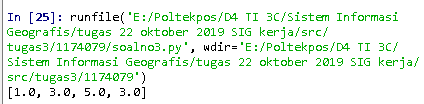
\includegraphics[width=6cm]{figures/Tugas3/1174079/soal3.png}
		\centering
		\caption{Gambar Soal 3}
	\end{figure}
	\item Nomor 4
	\lstinputlisting{src/tugas3/1174079/soalno4.py}
	\begin{figure}[H]
		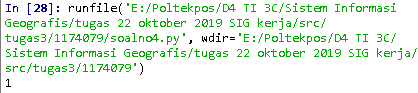
\includegraphics[width=6cm]{figures/Tugas3/1174079/soal4.png}
		\centering
		\caption{Gambar Soal 4}
	\end{figure}
	\item Nomor 5
	\lstinputlisting{src/tugas3/1174079/soalno5.py}
	\begin{figure}[H]
		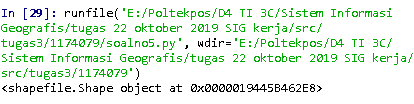
\includegraphics[width=6cm]{figures/Tugas3/1174079/soal5.png}
		\centering
		\caption{Gambar Soal 5)}
	\end{figure}
	\item Nomor 6
	\lstinputlisting{src/tugas3/1174079/soalno6.py}
	\begin{figure}[H]
		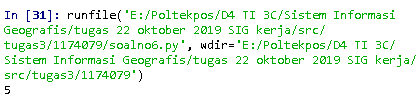
\includegraphics[width=6cm]{figures/Tugas3/1174079/soal6.png}
		\centering
		\caption{Gambar Soal 6}
	\end{figure}
	\item Nomor 7
	\lstinputlisting{src/tugas3/1174079/soalno7.py}
	\begin{figure}[H]
		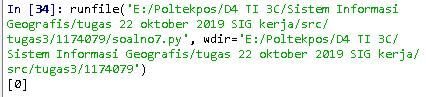
\includegraphics[width=6cm]{figures/Tugas3/1174079/soal7.png}
		\centering
		\caption{Gambar Soal 7)}
	\end{figure}
	\item Nomor 8
	\lstinputlisting{src/tugas3/1174079/soalno8.py}
	\begin{figure}[H]
		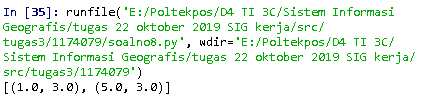
\includegraphics[width=6cm]{figures/Tugas3/1174079/soal8.png}
		\centering
		\caption{Gambar Soal 8)}
	\end{figure}
	\item Nomor 9
	\lstinputlisting{src/tugas3/1174079/soalno9.py}
	\begin{figure}[H]
		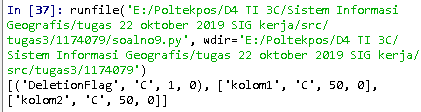
\includegraphics[width=6cm]{figures/Tugas3/1174079/soal9.png}
		\centering
		\caption{Gambar Soal 9}
	\end{figure}
	\item Nomor 10
	\lstinputlisting{src/tugas3/1174079/soalno10.py}
	\begin{figure}[H]
		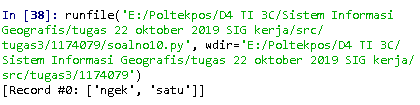
\includegraphics[width=6cm]{figures/Tugas3/1174079/soal10.png}
		\centering
		\caption{Gambar Soal 10 }
	\end{figure}
	\item Nomor 11
	\lstinputlisting{src/tugas3/1174079/soalno11.py}
	\begin{figure}[H]
		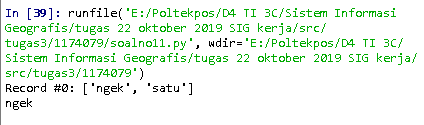
\includegraphics[width=6cm]{figures/Tugas3/1174079/soal11.png}
		\centering
		\caption{Gambar Soal 11 }
	\end{figure}
\end{enumerate}
\subsection{Link}
https://youtu.be/WM1Mg8TGOdY